\chapter{把多张图组织成论文组图}
\usetikzlibrary{patterns}
\providecommand{\ding}[1]{$\times$}
\providecommand{\sout}[1]{\leavevmode\begingroup\sbox0{#1}\hbox{\copy0\kern-\wd0\rule[0.5ex]{\wd0}{0.4pt}}\endgroup}

材料学博士生小周正在撰写一篇平面钙钛矿太阳能电池界面钝化改性的论文。她手头已经有四张分别做好的单图：一张展示器件七层堆叠关系的截面结构示意图、一张展示各功能层纵截面形貌的示意图、一张对照与改性器件的电流密度—电压（$J\text{--}V$）曲线图，以及一张连续光照下归一化光电转换效率（PCE）随时间变化的运行稳定性曲线图。为了拼出论文的核心结果图（Figure 2），她把这四张图片按文件夹里的排序拖进同一页演示文稿，随手拉动四角把画面凑成两行两列，另存为一张大图发给导师。

第二天早上，导师退回的手稿上只留了三行批注：“左下图蓝线和右下图红线，到底哪条是对照？”“b 图被拉扁了？”“缩到版面宽度后，左下图的坐标轴数字还看得清吗？”

小周把那页拼图按期刊双栏宽度（$174\ \text{mm}$）100\% 缩放打印在 A4 纸上，拿着尺子逐一比对，才发现问题远不止导师指出的三处：四个面板的编号分别写成了大写“A”、带括号的“(b)”、带句点的“c.”，第四个面板干脆漏了字母；左下图的刻度文字缩成了不到 $5\ \text{pt}$；两张数据图不仅配色前后冲突，而且全用实线绘制，黑白打印后无法区分组别；左右两个数据面板的坐标轴底边还上下错开了三毫米多。

论文组图不是四张单图的收纳盒，而是围绕一个核心问题展开的视觉论证。本章从这页被退回的初稿出发，逐步拆解如何先写论证问题再分配面板、如何在最终印刷尺寸上规划网格、如何让不同来源的面板说同一种视觉语言、如何对齐坐标轴框与编号留白，并结合 \scidraw{} 的组图与图注工具完成从杂乱拼图到可核查终稿的全过程。

\section{先写问题，再分配面板}

在打开排版工具画网格之前，作者首先要回答一个基本问题：为什么这几张子图必须合并成同一张大图（Figure 2），而不是拆成四张独立的单图？

在学术论文中，多面板组图（multi-panel figure）存在的唯一理由，是\textbf{多个面板共同回答同一个上位科学问题，且读者需要在同一视野内跨面板比对不同维度的证据}（Rougier 等，2014；Jambor 等，2021）。如果几张图各自讨论互不相干的话题，硬拼在一起只会分散读者的注意力；反过来，如果它们共同支撑一条完整的论证链条，把它们组织在同一张双栏画布上，就能让审稿人在一次视线扫视中完成“理解改性方案—确认截面层序—核对初始效率—检验长期稳定性”的闭环。

初学者在组织组图时，最容易掉进三个误区：
\begin{itemize}
\item \textbf{按实验先后顺序堆砌日记：}把课题先测的样品表征放前面、后测的放后面，缺乏统一的核心论点，读者看完八个面板也不知道这一节到底要证明什么。
\item \textbf{不同面板重复证明同一件事：}例如用两张高度同质的曲线或柱状图反复展示同一个效率提升数值，既浪费宝贵的版面，又挤压了关键证据的展示面积。
\item \textbf{把无关的常规质控图塞进主图：}生怕审稿人觉得工作量不够，把所有常规物相确认图全塞进一张大图，导致每个面板缩得像邮票，关键曲线的细节反而看不清。
\end{itemize}

要避开这些误区，组图的第一步应当是先写下整张组图要回答的\textbf{主问题}，再为每个候选面板分配明确的\textbf{子问题与证据角色}。在本章案例中，Figure 2 要回答的主问题是一句可检验的问句：

\begin{BookNote}
\textbf{Figure 2 主问题：}在钙钛矿与空穴传输层界面引入钝化层，是否同时提高了平面器件的初始光电转换效率和运行稳定性？
\end{BookNote}

围绕这一个主问题，手头的四个面板立即有了各司其职的论证分工（图~\ref{fig:ch09-01}）：
\begin{itemize}
\item \textbf{面板 a（器件结构示意）：}回答“改了什么”。它交代平面正置（n-i-p）器件自下而上的七层结构（玻璃 / FTO / $\text{SnO}_2$ / 钙钛矿 / 钝化层 / spiro-OMeTAD / Au）与入射光方向，标出新增钝化层所在的界面位置，属于提供概念背景的\textbf{解释性面板}。
\item \textbf{面板 b（截面形貌示意）：}回答“各功能层是否连续、层序如何对应”。它为左侧抽象层叠框提供纵截面形貌参照（本教学案例采用图像模型生成的类电镜截面示意并在面板内声明；真实论文中对应同批器件的实际截面扫描电镜图像）。
\item \textbf{面板 c（$J\text{--}V$ 特性曲线）：}回答“初始效率是否提高、提高来自开路电压（$V_{\text{oc}}$）、短路电流密度（$J_{\text{sc}}$）还是填充因子（FF）”。它提供初始光电转换性能对比的\textbf{定量数据证据}。
\item \textbf{面板 d（归一化 PCE 随时间变化）：}回答“连续运行条件下稳定性是否提高、效率降至初始值 80\% 的时间（$T_{80}$）延长了多少”。它提供长期运行稳定性的\textbf{定量数据证据}。
\end{itemize}

\begin{figure}[htbp]\centering
\resizebox{\linewidth}{!}{% FIG ch09-01 panel argument map (Chinese)
\begin{tikzpicture}[
  x=1mm, y=1mm,
  font=\sffamily\small,
  text=BookInk,
  mainbox/.style={
    draw=BookTeal, line width=0.6pt, rounded corners=2pt,
    fill=BookPale, align=center, text width=150mm, inner sep=3mm,
  },
  explain/.style={
    draw=BookRule, fill=BookRule!35, rounded corners=2pt,
    align=left, text width=38mm, inner sep=2.5mm, minimum height=18mm,
  },
  data/.style={
    draw=BookInk!50, fill=white, rounded corners=2pt,
    align=left, text width=38mm, inner sep=2.5mm, minimum height=18mm,
  },
  moved/.style={
    draw=BookInk!40, dashed, rounded corners=2pt,
    align=left, text width=155mm, inner sep=2.5mm,
  },
]
  \node[mainbox] (q) at (87, 58)
    {主问题：界面钝化改性是否同时提高了初始效率和运行稳定性？};
  \foreach \i/\x/\t in {
    a/20/示意, b/62/形貌, c/104/性能, d/146/稳定性} {
    \node[explain] (\i) at (\x, 32) {
      \textbf{\i}\par
      回答：改了什么 / 层序是否连续 / 初始效率 / 运行稳定性\par
      \scriptsize 证据类型：\t
    };
  }
  \draw[-{Stealth[length=2mm]}, BookInk!60, thick] (q.south) -- (a.north);
  \draw[-{Stealth[length=2mm]}, BookInk!60] (a.east) -- (b.west);
  \draw[-{Stealth[length=2mm]}, BookInk!60] (b.east) -- (c.west);
  \draw[-{Stealth[length=2mm]}, BookInk!60] (c.east) -- (d.west);
  \node[moved] at (87, 8) {
    候选但移出（\textbf{示例}）：XRD 图谱 $\rightarrow$ 补充材料（不直接回答主问题）
  };
\end{tikzpicture}
}
\caption{Figure 2 的论证分工。每个面板回答主问题下的一个子问题；不直接服务于主问题的候选面板移到补充材料。}\label{fig:ch09-01}
\end{figure}

写清面板角色后，\textbf{面板的排列顺序也就随之确定：阅读顺序必须与论证顺序一致}。横排科技论文的读者默认沿“从左到右、从上到下”的路径扫视组图（Jambor 等，2021）。把交代“是什么”的解释性面板（\textbf{a}、\textbf{b}）放在上排，把证明“效果怎么样”的数据面板（\textbf{c}、\textbf{d}）放在下排，读者的视线沿 $\textbf{a} \rightarrow \textbf{b} \rightarrow \textbf{c} \rightarrow \textbf{d}$ 推进时，刚好顺着“结构设计 $\rightarrow$ 截面层序 $\rightarrow$ 初始性能 $\rightarrow$ 运行稳定性”的逻辑阶梯前进，无需在版面上来回折返。

这套分工表还能帮作者果断做减法：\textbf{把没有直接论证分工的面板移到补充材料}。判断一个候选面板去留的标准只有一条：\textbf{拿掉它之后，这张图的主问题还能不能完整回答？} 如图~\ref{fig:ch09-01} 底部虚线框所示，假设手头还有一张用于确认薄膜成相的 X 射线衍射（XRD）图谱（此处仅作方法示例，本案例无实测 XRD 数据），它回答的是“是否形成了目标钙钛矿晶相、有无杂相峰”，属于材料制备的基础物相质控，并不直接回答“界面钝化是否同时提高初始效率与运行稳定性”。将其移入补充材料（Supplementary Information），在正文中用半句话引用即可，从而把主图空间留给四个核心面板。

在这一步，作者可以把研究主问题与手头已有的单图清单发给 AI，让它协助梳理面板分工与排列顺序：

\begin{Prompt}
我准备制作钙钛矿太阳能电池论文的 Figure 2（双栏宽 174 mm）。
主问题：钙钛矿/空穴传输层界面钝化是否同时提高了初始效率和运行稳定性？
候选单图：(1) 器件层状结构示意；(2) 截面形貌图；(3) 对照与改性 J-V 曲线；
(4) 连续光照 1000 h 归一化 PCE 曲线；(5) 薄膜 XRD 物相确认图。
请列出每张图回答的子问题与证据类型，指出哪张图不直接支撑主问题、建议移至
补充材料，并按左到右、上到下的阅读习惯给出其余面板的排列顺序。
\end{Prompt}

AI 能根据任务描述快速列出面板分工候选，并指出第 (5) 项 XRD 图谱不直接服务于主问题。但作者必须清楚边界：\textbf{AI 不能判断现有证据在科学上是否充分，也不能替你决定取舍哪些实验结果}；哪些数据必须如实展示、哪些基础表征移入补充材料，必须由作者按领域规范拍板。

\section{在最终尺寸上规划网格}

定下面板顺序后，第二步是在\textbf{目标期刊的最终印刷尺寸}上规划网格，而不是“先按默认大尺寸画好单图，最后拖进拼图画布缩小”。

为什么“先做大图再缩小”是组图字号崩盘的头号原因？我们可以算一笔具体的账。Python Matplotlib 等绘图工具新建画布时的默认尺寸通常是 $8 \times 6\ \text{in}$（即 $203.2 \times 152.4\ \text{mm}$），默认文字字号为 $10\ \text{pt}$。在电脑屏幕上单独查看时，字号显得很合适。然而，期刊印刷版面的栏宽是固定的：例如 Springer 与 Cell 旗下多数期刊（以及 \scidraw{} 组图工具的对应预设）单栏宽约为 $84\text{--}85\ \text{mm}$，双栏通栏宽为 $174\ \text{mm}$；Nature 系列单栏宽为 $89\ \text{mm}$，双栏通栏宽为 $183\ \text{mm}$。

当两张图横向并排放入 $174\ \text{mm}$ 宽的双栏画布、中间留出 $6\ \text{mm}$ 间距时，每个格子分到的宽度只有 $(174 - 6) / 2 = 84\ \text{mm}$。把一张 $203.2\ \text{mm}$ 宽的图像缩进 $84\ \text{mm}$ 的格子里，线性缩放系数为：
\[
s = \frac{84\ \text{mm}}{203.2\ \text{mm}} \approx 0.413
\]
原图中 $10\ \text{pt}$ 的刻度与轴标题会同步缩小到约 $4.1\text{--}4.5\ \text{pt}$，原本 $0.8\ \text{pt}$ 的坐标轴线则会缩成约 $0.33\ \text{pt}$ 的细丝。

学术期刊对配图在\textbf{最终印刷尺寸下}的字号有明确规定：Nature 官方图片规范要求普通文字为 $5\text{--}7\ \text{pt}$、面板字母为 $8\ \text{pt}$ 粗体小写；而按更稳妥的跨期刊标准（如 Springer 预设与常规审稿阅读体验），正图中的所有刻度、轴标题与标注文字建议不小于 $8\ \text{pt}$，面板字母采用 $10\ \text{pt}$ 粗体（各期刊现行作者指南可能更新，动工前与投稿前均须核对目标期刊网站规定）。无论投哪家期刊，$4.5\ \text{pt}$ 的文字都远低于可读下限。

要根除这一问题，唯一可靠的做法是：\textbf{先确定整张组图的物理毫米尺寸与网格划分，再让每个数据面板直接按最终格子尺寸（毫米除以 $25.4$ 换算为英寸）出图，使拼合时的缩放系数严格等于 $1.0$。} 即使后续改投栏宽 $183\ \text{mm}$、字号要求 $5\text{--}7\ \text{pt}$ 的期刊，也只需修改脚本中的画布宽度和字号常数重新运行导出，而不应直接拉伸已有位图。

规划网格时，还必须兼顾各面板内容的\textbf{天然宽高比}。示意图、截面电镜图与折线图的最佳长宽比例并不相同。图~\ref{fig:ch09-02} 在 $174\ \text{mm}$ 最终印刷宽度下对比了两种候选网格方案。

\begin{figure}[htbp]\centering
\resizebox{0.84\linewidth}{!}{% FIG ch09-02 layout wireframes (Chinese)
\begin{tikzpicture}[
  x=1mm, y=1mm,
  font=\sffamily\footnotesize,
  text=BookInk,
  frame/.style={draw=BookInk!70, line width=0.5pt},
  cell/.style={draw=BookRule, fill=BookPale!50, line width=0.3pt},
  bad/.style={pattern=north east lines, pattern color=BookInk!25},
]
  \node[anchor=west, font=\bfseries] at (0, 125) {方案 A（2$\times$2 等分）};
  \draw[frame] (0, 68) rectangle (174, 122);
  \node[anchor=south] at (87, 122) {174 mm};
  \foreach \x/\y/\w/\h in {0/68/84/53, 90/68/84/53, 0/10/84/53, 90/10/84/53} {
    \draw[cell] (\x,\y) rectangle (\x+\w,\y+\h);
  }
  \draw[bad] (90,68) rectangle (174,121);
  \node[anchor=west, text=BookTeal] at (92, 95) {需拉伸 \ding{55}};
  \node[anchor=west, align=left, text width=84mm] at (0, 4) {
    优点：网格简单。问题：b 填满格子需改变宽高比。
  };

  \node[anchor=west, font=\bfseries] at (0, 248) {方案 B（采用）};
  \draw[frame] (0, 186) rectangle (174, 240);
  \draw[cell] (0,214) rectangle (84,264);
  \draw[cell] (90,214) rectangle (174,264);
  \draw[cell] (0,154) rectangle (84,210);
  \draw[cell] (90,154) rectangle (174,210);
  \draw[BookTeal, dashed, line width=0.4pt] (12,154) -- (12,210);
  \draw[BookTeal, dashed, line width=0.4pt] (102,154) -- (102,210);
  \node[text=BookTeal, font=\scriptsize] at (57,152) {对齐};
  \node[text=BookTeal, font=\scriptsize] at (147,152) {对齐};
  \node[anchor=west, align=left, text width=90mm] at (0, 178) {
    上排 84$\times$50 mm；下排 84$\times$56 mm；列距 6 mm，行距 8 mm。
  };
  \node[anchor=west, align=left, text width=84mm] at (0, 168) {
    优点：保留 b 比例；c、d 轴框对齐。问题：需预先算好格子尺寸。
  };
\end{tikzpicture}
}
\caption{在最终印刷宽度上比较两个网格方案。方案 A 等分格子，截面图需拉伸才能填满；方案 B 按内容比例分配高度，并把两个数据面板的坐标轴框对齐。尺寸单位为 mm。}\label{fig:ch09-02}
\end{figure}

图~\ref{fig:ch09-02} 下方的\textbf{方案 A（$2 \times 2$ 等分）}将 $174 \times 114\ \text{mm}$ 画布机械地四等分为 $84 \times 53\ \text{mm}$ 的格子。问题在于：面板 \textbf{a}（结构示意）底图宽高比约为 $16:10$，且右侧需留出约 35\% 宽度标注七层名称；面板 \textbf{b}（截面形貌）宽高比严格为 $3:2$；下排面板 \textbf{c}、\textbf{d} 则需在绘图框外留出纵轴与横轴标题空间。若强行让面板 \textbf{b} 填满方案 A 的等分格子（图中斜线阴影区），就必须非等比拉伸图像，直接扭曲截面层厚比与柱状晶粒的几何形貌。

图~\ref{fig:ch09-02} 上方的\textbf{方案 B（按内容比例分配，本例采用）}在 $174\ \text{mm}$ 宽、总高不超过 $120\ \text{mm}$ 的约束下，按内容特征分配空间：上排解释组（\textbf{a}、\textbf{b}）规划为 $84 \times 50\ \text{mm}$，图像按原始宽高比置入并自然留白；下排数据组（\textbf{c}、\textbf{d}）规划为 $84 \times 56\ \text{mm}$；列间距设为 $6\ \text{mm}$，上下排之间留出 $8\ \text{mm}$ 行距以区分“解释”与“数据”两组；同时将 \textbf{c}、\textbf{d} 的坐标轴框严格对齐（图中青色虚线）。

\section{让面板说同一种语言}

当组图中的四个面板分别来自不同工具——例如面板 \textbf{a}、\textbf{b} 底图由图像生成工具绘制，面板 \textbf{c}、\textbf{d} 由 Python 脚本绘制——最容易出现“四个面板像从四篇不同文章里剪贴过来”的拼凑感。要让所有面板融为一个整体，必须统一五项视觉语法。

\textbf{第一，统一无衬线字体，压缩字号与线宽层级。}
全图只用同一种无衬线字体（英文用 Helvetica、Arial 或 TeX Gyre Heros，中文配黑体如思源黑体或 FandolHei），绝不在示意图里用衬线体、到了数据图里又换无衬线体。字号层级只设两档：四个面板编号字母（\textbf{a}–\textbf{d}）统一用 $10\ \text{pt}$ 粗体；其余全部文字（轴标题、刻度、曲线旁注、层名与面板内声明）统一用 $8\ \text{pt}$。坐标轴框与刻度线宽统一为 $0.6\ \text{pt}$，数据曲线线宽统一为 $1.2\ \text{pt}$，参考线与水平背景网格线则采用更轻的视觉权重（$1.0\ \text{pt}$ 浅灰点线与 $0.5\ \text{pt}$ 极浅灰细线）。

\textbf{第二，让颜色语义跨面板贯穿。}
颜色在组图中是代表特定实验组别的视觉代词（Wong，2011；Crameri 等，2020）。一旦在某个面板中定义了颜色含义，就必须贯彻到底。在本例中，“界面钝化改性”是贯穿全图的主线：面板 \textbf{a} 的器件结构示意图里，钙钛矿吸光层上方的极薄钝化层采用青色（\texttt{\#1B7F86}），右侧“钝化层”三字也用同款青色标注；到了下排的数据面板 \textbf{c} 和 \textbf{d}，“改性”组曲线与旁注继续使用同一个青色（\texttt{\#1B7F86}），无钝化层的“对照”组则统一使用中性深灰色（\texttt{\#6E6E6E}）。读者在面板 \textbf{a} 建立“青色 = 钝化改性”的印象后，视线移到 \textbf{c}、\textbf{d} 时无需寻找图例就能直接读懂曲线身份。

\textbf{第三，用“颜色 + 线型”双重编码，保障灰度打印与色觉无障碍。}
单靠颜色区分组别并不可靠。深灰色（\texttt{\#6E6E6E}）与青色（\texttt{\#1B7F86}）的明度非常接近，如果两条曲线都画成实线，一旦转为灰度图或用黑白打印机输出，两条线就会变成深浅几乎一样的灰线；色觉差异读者同样需要颜色之外的几何线索（Machado 等，2009）。因此，我们在颜色之外叠加\textbf{线型编码}（图~\ref{fig:ch09-05}）：改性组固定为\textbf{青色实线}，对照组固定为\textbf{灰色虚线}（线段与空白比 $4:2$），面板 \textbf{d} 中表示初始值 80\% 的参考线则采用\textbf{浅灰色（\texttt{\#9A9A9A}）点线}（$1:3$）。这样即使整张图变成纯黑白稿，实线、虚线与点线依然一清二楚。

\begin{figure}[htbp]\centering
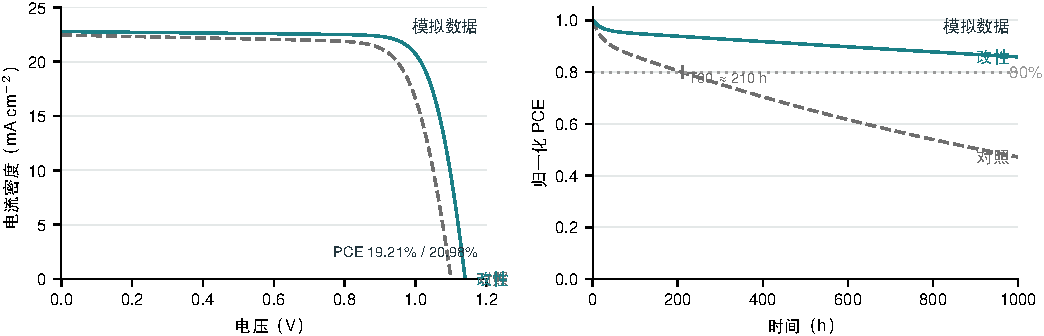
\includegraphics[width=\linewidth]{figures/ch09/ch09-05-data-panels-zh.pdf}
\caption{按最终尺寸（每面板 $84 \times 56\ \text{mm}$）绘制的两个数据面板。(c) 对照（灰色虚线）与改性（青色实线）的模拟 $J\text{--}V$ 曲线。(d) 归一化 PCE 随时间变化，点线为 80\%。两组同时由颜色和线型区分，灰度打印仍可分辨；曲线由单二极管模型与给定衰减函数生成，为模拟教学数据。注意左图右下角：若将直接标注机械绑定在曲线末点，两条在 $V_{\text{oc}}$ 处归零的曲线会导致“对照”“改性”与横轴末位刻度重叠，这一问题在终稿（图~\ref{fig:ch09-07}）中修正。}\label{fig:ch09-05}
\end{figure}

\textbf{第四，用直接标注替代图例框，并排查文字与曲线的几何碰撞。}
在只有两条曲线的数据图中，去掉带边框的图例盒、直接在曲线旁写上同色的“改性”与“对照”，能省去视线在图例与曲线之间来回跳跃的负担。

但直接标注绝不能在脚本里简单写成“把标签放在最后一个数据点 \texttt{(x[-1], y[-1])} 处”。观察图~\ref{fig:ch09-05} 的实际画面，就能看到自动贴末点带来的真实碰撞问题：在左图（面板 \textbf{c}）中，对照与改性两条 $J\text{--}V$ 曲线都在右侧陡降，分别于开路电压 $1.100\ \text{V}$ 和 $1.140\ \text{V}$ 处交于横轴（$J = 0$）。把标签绑在曲线末端，导致“对照”和“改性”两个词在右下角 $1.2\ \text{V}$ 刻度处严重重叠，而右下方的“PCE 19.21\% / 20.98\%”又被灰色虚线直接穿过；在右图（面板 \textbf{d}）中，右端的“改性”“80\%”“对照”紧贴曲线末端，且“$\text{T80} \approx 210\ \text{h}$”压在了虚线上。

这说明\textbf{直接标注必须根据曲线走势人工放置在邻近的空白通带（open band）内，并放大到 200\% 复核}。在终稿（图~\ref{fig:ch09-07}）中，我们将面板 \textbf{c} 的“改性”和“对照”移到陡降段左侧的开阔区（分别为 $(0.96\ \text{V},\ 15.5\ \text{mA cm}^{-2})$ 与 $(1.00\ \text{V},\ 5.0\ \text{mA cm}^{-2})$），把 PCE 汇总移到左下角 $(0.03,\ 0.04)$；将面板 \textbf{d} 的标注移到各自曲线上方的空白带并加半透明白底衬垫，彻底消除了压线与撞字。

\textbf{第五，统一物理量单位与面板内真实性声明。}
删除单图顶部与图注重复的独立标题（如“J-V curve”“Stability test”）；单位格式全图统一为 $\text{V}$、$\text{mA cm}^{-2}$、$\text{h}$，二氧化锡下标用数学模式排为 $\mathrm{SnO_2}$；并在面板内部直接标出“不按比例”（\textbf{a}）、“模型生成示意，非显微图像”（\textbf{b}）和“模拟数据”（\textbf{c}、\textbf{d}），确保单面板被截图放进幻灯片或海报时声明不丢失。

\section{对齐、编号与留白}

将四个面板排入同一张画布时，决定版面是否整洁专业的核心是三件事：对齐、编号与留白。

\textbf{第一件事：对齐坐标轴框（spine box），而不是对齐图片外框（bounding box）。}
面板 \textbf{c} 的纵轴刻度是两位数整数（\texttt{0–25}）且轴标题含括号与上标，面板 \textbf{d} 的纵轴刻度是一位小数（\texttt{0.0–1.0}）。如果把两张开启了自动紧凑裁剪（\texttt{bbox\_inches='tight'}）的单图拖进画布并对齐图片左边缘，由于两图左侧文字宽度不同，里面的坐标轴矩形框反而会一左一右、一高一低。

读者扫视并排图表时，眼睛寻找的基准线是实实在在画出来的坐标轴线。因此，合成组图时不应使用弹性自适应布局（\texttt{tight\_layout}），而应\textbf{以毫米为单位直接固定每个面板框在画布上的绝对矩形坐标}。例如在终稿（图~\ref{fig:ch09-07}）的 $174.0 \times 116.0\ \text{mm}$ 画布上，左起先留 $13.0\ \text{mm}$ 给左列纵轴标题与刻度，左列（面板 \textbf{a} 外框与面板 \textbf{c} 坐标轴框）统一占据 $x = 13.0\text{--}82.0\ \text{mm}$（宽 $69.0\ \text{mm}$）；中间留 $6.0\ \text{mm}$ 列间距和 $13.0\ \text{mm}$ 右列纵轴走廊，右列（面板 \textbf{b} 外框与面板 \textbf{d} 坐标轴框）统一占据 $x = 101.0\text{--}170.0\ \text{mm}$（宽 $69.0\ \text{mm}$），最右侧留 $4.0\ \text{mm}$ 边距并将末位刻度“1.2”与“1000”设为右对齐内收；下排 \textbf{c}、\textbf{d} 坐标轴框底边统一固定在 $y = 11.0\ \text{mm}$、高 $46.0\ \text{mm}$，并用脚本断言（\texttt{assert}）自动校验四框边界坐标完全相等。

\textbf{第二件事：面板字母统一样式、位置与基线，置于画布外侧白底走廊。}
面板编号字母是正文、图注与画面之间的唯一定位路标，必须遵守四条规则：
\begin{enumerate}
\item \textbf{样式全图唯一：}按目标期刊规范统一格式（本例采用 $10\ \text{pt}$ TeX Gyre Heros Bold 粗体无衬线小写 \textbf{a}–\textbf{d}，不加括号和句点）。
\item \textbf{对齐面板左缘与同行基线：}左列字母 \textbf{a}、\textbf{c} 左缘对齐 $x = 13.0\ \text{mm}$，右列字母 \textbf{b}、\textbf{d} 左缘对齐 $x = 101.0\ \text{mm}$；上排 \textbf{a}、\textbf{b} 与下排 \textbf{c}、\textbf{d} 各自共享同一条水平基线（均位于面板框顶边上方 $1.0\ \text{mm}$）。
\item \textbf{顶部预留安全带：}在画布顶部专门留出 $5.0\ \text{mm}$ 白边走廊，防止上排面板上方的字母被裁切。
\item \textbf{不压深色图像内部：}字母一律放在面板框外侧的白底走廊上，避免压在面板 \textbf{b} 顶部的暗黑背景上导致看不清。
\end{enumerate}

\textbf{第三件事：用留白传递分组信息，严守图像面板原始宽高比。}
按照视觉接近性原则，不同功能组之间的留白应大于同组内部：本例同排左右列间距为 $6.0\ \text{mm}$，而上排解释组（\textbf{a}、\textbf{b}）与下排数据组（\textbf{c}、\textbf{d}）之间的行距加大为 $8.0\ \text{mm}$。同时，图像面板绝不能为了填满格子而设置非等比拉伸（\texttt{aspect='auto'}）：在 $69.0\ \text{mm}$ 统一列宽下，面板 \textbf{a}（源像素 $1586 \times 992$）自然高度为 $43.2\ \text{mm}$，面板 \textbf{b}（源像素 $1536 \times 1024$）自然高度为 $46.0\ \text{mm}$；让两面板顶边齐平于 $y = 111.0\ \text{mm}$，面板 \textbf{a} 底部自然留出的 $2.8\ \text{mm}$ 白边刚好安放入射光与“不按比例”标签。

\section{完整案例：钙钛矿 Figure 2 从杂乱到可投稿前稿}

现在把前面四节的原则串起来，完整走一遍平面钙钛矿太阳能电池 Figure 2 从材料准备、任务书、底图生成、初稿排错到终稿复现的全过程（本案例与第 12、13 章共用同一套模拟数据）。

\subsection*{第一步：清点材料与模拟参数}

教学设定比较平面正置（n-i-p）对照器件与界面钝化改性器件。自下而上层序为：玻璃 / FTO / $\text{SnO}_2$（示意厚度约 $30\ \text{nm}$）/ 钙钛矿（约 $500\ \text{nm}$）/ 钝化层（仅改性组，极薄）/ spiro-OMeTAD（约 $200\ \text{nm}$）/ Au（约 $80\ \text{nm}$），光从玻璃侧入射。不指定具体钙钛矿组分与钝化分子，也不报告任何真实器件测试结果。

四项材料中，M1（面板 \textbf{a} 结构示意）和 M2（面板 \textbf{b} 类 SEM 截面图样）由图像模型生成无字底图；M3（面板 \textbf{c} $J\text{--}V$ 曲线）由 Python 脚本按单二极管方程 $J = J_{\text{L}} - J_0[\exp((V + J R_{\text{s}})/(n V_{\text{T}})) - 1] - (V + J R_{\text{s}})/R_{\text{sh}}$ 在 $25\ ^\circ\text{C}$（$V_{\text{T}} = 0.025693\ \text{V}$）、AM1.5G（$100\ \text{mW cm}^{-2}$）下以 $0.5\ \text{mV}$ 步长二分法求解，仅模拟单一扫描方向，不模拟迟滞；M4（面板 \textbf{d} 稳定性曲线，$0\text{--}1000\ \text{h}$，步长 $10\ \text{h}$）按双指数衰减函数 $y(t) = [1 - b(1 - e^{-t/20})]e^{-t/\tau}$ 生成（对照取 $b = 0.08, \tau = 1500\ \text{h}$；改性取 $b = 0.04, \tau = 9000\ \text{h}$）。每组仅有一条代表性模拟曲线，参数与计算指标见表~\ref{tab:ch09-sim}。

\begin{table}[htbp]\centering\footnotesize
\setlength{\tabcolsep}{3.5pt}
\renewcommand{\arraystretch}{1.15}
\caption{面板 c、d 的单二极管模拟参数与计算指标（模拟教学数据）。}\label{tab:ch09-sim}
\begin{tabularx}{\linewidth}{@{}lcccYY@{}}
\toprule
\textbf{组别} & $J_{\text{L}}$ / 目标 $V_{\text{oc}}$ & $n$ & $R_{\text{s}}$ / $R_{\text{sh}}$ ($\Omega\cdot\text{cm}^2$) & \textbf{计算 $J_{\text{sc}}$ / $V_{\text{oc}}$ / FF} & \textbf{计算 PCE 与 $T_{80}$} \\
\midrule
对照 & $22.5\ \text{mA cm}^{-2}$ / $1.10\ \text{V}$ & 1.6 & $2.5$ / $1500$ & $22.46\ \text{mA cm}^{-2}$ / $1.100\ \text{V}$ / $0.777$ & $19.21\%$；$T_{80} = 210\ \text{h}$ \\
改性 & $22.8\ \text{mA cm}^{-2}$ / $1.14\ \text{V}$ & 1.5 & $2.0$ / $3000$ & $22.78\ \text{mA cm}^{-2}$ / $1.140\ \text{V}$ / $0.808$ & $20.98\%$；$T_{80} > 1000\ \text{h}$ \\
\bottomrule
\end{tabularx}
\end{table}

\begin{BookNote}
\textbf{为什么面板 b 不用开放许可的真实 SEM 图？} 公开文献中虽有 CC BY 4.0 许可的真实钙钛矿 SEM 图像，如 Burkitt 等（2018）图 6（使用 Jeol JSM-7800F 拍摄的旋涂与狭缝涂布钙钛矿层俯视 SEM 图，标有 $10\ \mu\text{m}$ 与 $1\ \mu\text{m}$ 比例尺），但该文器件是\textbf{介孔 $\text{TiO}_2$ 支架 + 甲胺铅碘氯钙钛矿、最佳稳定效率约 $7\%$}，与本例平面 $\text{SnO}_2$ 器件和模拟数值毫无关系。若将其放进本例 Figure 2，会让读者误以为形貌和性能来自同一批器件——这正是第 8 章所禁止的“来自不同样品的图像冒充同一来源”。因此本例面板 \textbf{b} 采用模型生成图样并在面板内标注“非显微图像”；真实研究中，面板 \textbf{b} 必须是同批器件的实际 SEM 采集，并按第 8 章保存原图与处理记录。
\end{BookNote}

\subsection*{第二步：组图任务书}

在 \scidraw{} 科研绘图向导（\sdtool{figure-workflow}）中选择“已有图片组图”路线，填写并下载保存完整任务书：

\begin{Prompt}
【用途与读者】论文 Figure 2，双栏通栏 174 mm 宽、高度不超过 120 mm；
读者为钙钛矿光伏方向的同行。目标期刊按 Springer 类要求准备：
文字不小于 8 pt（以期刊现行作者指南为准，投稿前再核对一次）。
【主问题】界面钝化改性是否同时提高了初始效率和运行稳定性？
【面板分工】
a 器件结构（改性器件；钝化层高亮）——回答“改了什么”。
b 截面形貌——回答“各层是否连续、钝化后形貌是否改变”。
  本书为模型生成示意，面板内标注“模型生成示意，非显微图像”。
c J–V 曲线（对照、改性）——回答“初始效率是否提高、提高来自哪个参数”。
d 归一化 PCE 随时间（对照、改性，0.8 参考线）——回答“稳定性是否提高”。
阅读顺序 a->b->c->d：先结构与形貌（是什么），再性能（怎么样）。
【布局】上排 a、b（解释性），下排 c、d（数据）；c、d 坐标轴框上下对齐、
高度相同；面板间距 6 mm；面板字母左上角，粗体小写，同一基线。
【统一规范】全图一种无衬线字体；刻度、轴标题、标注 8 pt，面板字母 10 pt 粗体；
轴线 0.6 pt，数据线 1.2 pt；对照 #6E6E6E 虚线，改性 #1B7F86 实线，
示意图中钝化层也用 #1B7F86；0.8 参考线为浅灰点线；直接标注，不用图例框；
单位写作 V、mA cm^-2、h。
【不可改变】c、d 的全部数值来自 sim-perovskite 数据文件；
b 的宽高比保持原样，不拉伸；c、d 面板内写“模拟数据”；a 写“不按比例”。
【交付】矢量 PDF（文字可选中）+ 600 dpi TIFF；处理记录；图注（作者补全版）。
【验收】在 174 mm 实际尺寸打印或 100% 缩放下：最小文字 >= 8 pt；
c、d 轴框对齐；四个面板字母样式一致；灰度打印能区分两组；
b 未变形；所有“模拟/模型生成/不按比例”标注在面板内可见。
\end{Prompt}

\subsection*{第三步：生成面板 a、b 底图并核查实际偏差}

面板 \textbf{a} 底图使用以下英文提示词生成（底图不含文字，右侧留出 35\% 空白供后期叠加层名）：

\begin{Prompt}
A clean, flat, two-dimensional scientific schematic of a planar thin-film solar
cell shown as a stack of horizontal layers in side view with a slight sense of
thickness. From bottom to top: a thick pale blue-grey translucent glass slab;
a thin light grey conductive layer; a very thin off-white layer; a thicker
dark reddish-brown absorber layer; an extremely thin teal layer (hex #1B7F86)
directly on top of the absorber; a pale yellow layer; and a thin gold metal
layer on top. Three simple upward-pointing light arrows below the glass,
pale yellow with grey outline. The stack occupies the left 65% of the canvas;
leave the right 35% empty white space for labels added later.
White background, vector illustration style, no gradients, no shadows,
no 3D rendering, no glow, no texture. Layers are not to scale but each layer is
clearly separated by a thin dark grey outline.
Absolutely no text, no letters, no numbers, no labels, no symbols, no scale bar.
Aspect ratio 16:10.
\end{Prompt}

将同一提示词连续生成三次（均为 $1586 \times 992\ \text{px}$，宽高比约 $1.599:1$，相对 $16:10$ 偏差 $-0.08\%$）。三次生成均正确呈现了自下而上的七层堆叠、玻璃下方三支向上的浅黄箭头以及干净无字的白底。但三次候选在细节上各有差异：第 2 次生成的青色钝化层偏厚（约 $29\ \text{px}$），弱化了“极薄界面层”的特征；第 3 次的青色偏亮（中值 \texttt{\#298F97}），且右侧空白占到了约 38.5\%。第 1 次生成右侧留白恰占约 35\%，青色层极薄且清晰，实测颜色中值 \texttt{\#20868D} 与目标色 \texttt{\#1B7F86} 三个通道仅差 $5\text{--}7$，故选作主图。同时核查可见主图仍有两处残余偏差：层内有轻微明暗渐变与细颗粒，未严格满足无渐变无纹理；正面玻璃层厚约 $148\ \text{px}$，略薄于钙钛矿层（约 $158\ \text{px}$）。我们在右侧空白处用引线叠加七层名称，并在右下角标明“不按比例”（图~\ref{fig:ch09-03}）。

\begin{figure}[htbp]\centering
\begin{tikzpicture}
\node[anchor=south west,inner sep=0] (img) at (0,0) {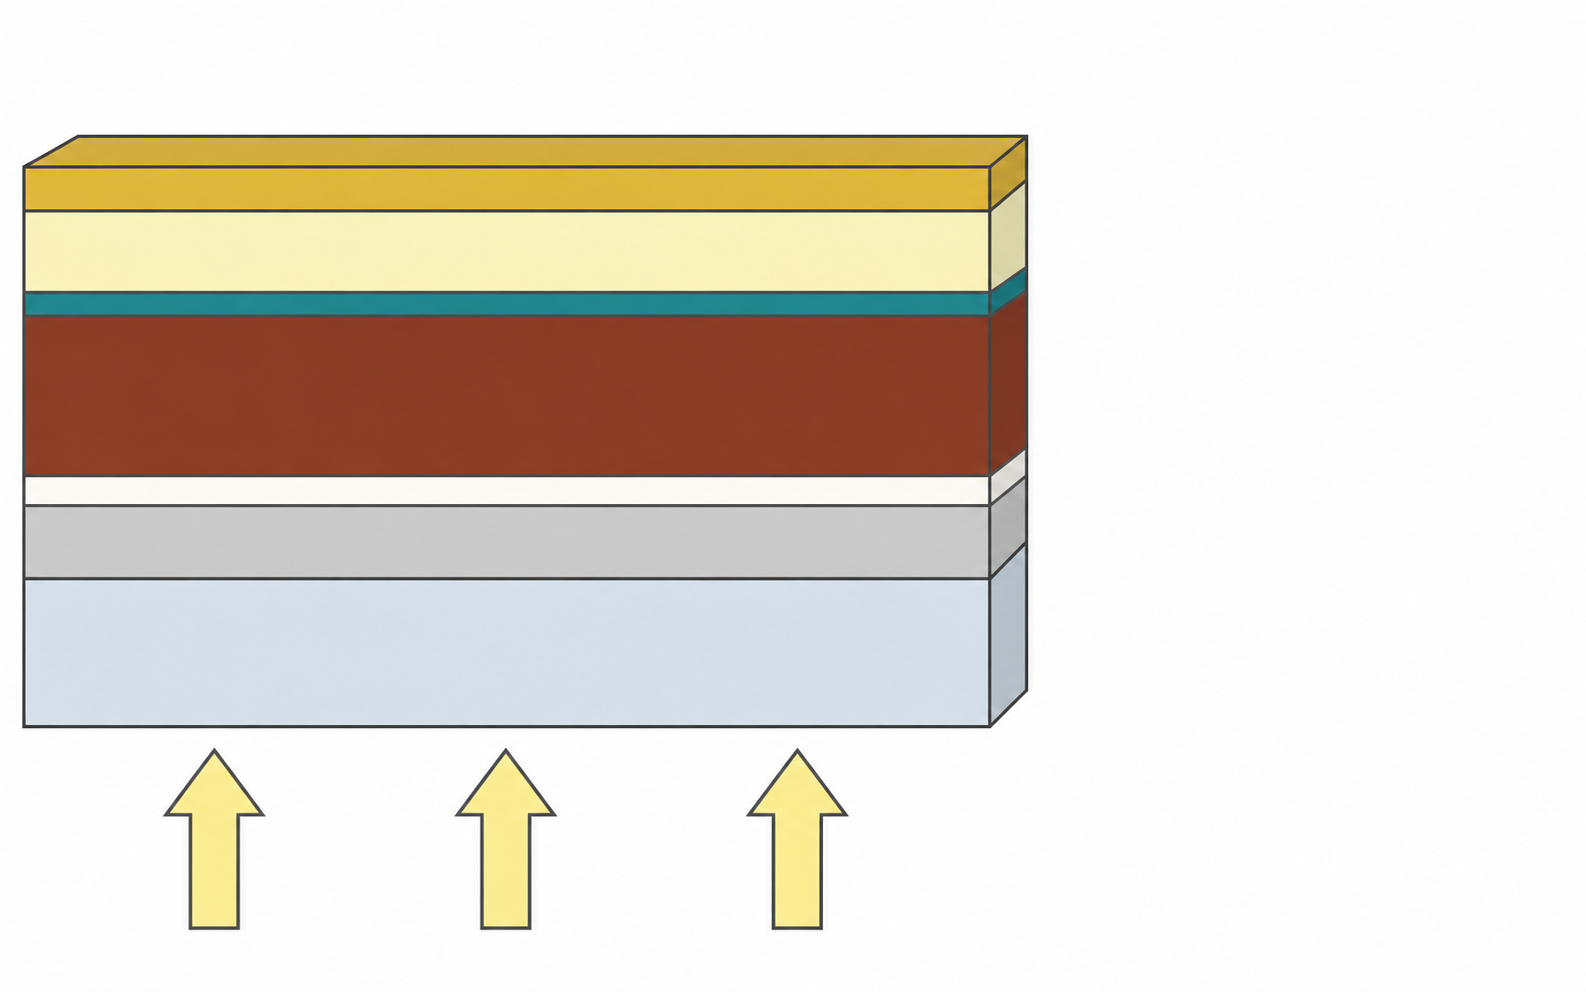
\includegraphics[width=0.86\linewidth]{figures/ch09/ch09-03-device-structure-base.png}};
\begin{scope}[x={(img.south east)},y={(img.north west)},font=\sffamily\footnotesize]
  \draw[BookInk!65,thin] (0.60,0.83) -- (0.69,0.86);
  \draw[BookInk!65,thin] (0.60,0.75) -- (0.69,0.76);
  \draw[BookTeal,thin] (0.60,0.698) -- (0.69,0.67);
  \draw[BookInk!65,thin] (0.60,0.60) -- (0.69,0.56);
  \draw[BookInk!65,thin] (0.60,0.505) -- (0.69,0.45);
  \draw[BookInk!65,thin] (0.60,0.45) -- (0.69,0.39);
  \draw[BookInk!65,thin] (0.60,0.33) -- (0.69,0.25);
  \node[anchor=west] at (0.70,0.86) {Au};
  \node[anchor=west] at (0.70,0.76) {spiro-OMeTAD};
  \node[anchor=west,text=BookTeal,font=\sffamily\footnotesize\bfseries] at (0.70,0.67) {钝化层};
  \node[anchor=west] at (0.70,0.56) {钙钛矿};
  \node[anchor=west] at (0.70,0.45) {$\mathrm{SnO_2}$};
  \node[anchor=west] at (0.70,0.39) {FTO};
  \node[anchor=west] at (0.70,0.25) {玻璃};
  \node[anchor=west] at (0.30,0.05) {入射光};
  \node[anchor=south east,text=BookInk!80] at (0.98,0.02) {不按比例};
\end{scope}
\end{tikzpicture}
\caption{改性器件结构示意（面板 a 底图由图像生成模型绘制，层名为后加标签）。钝化层与数据图中的“改性”使用同一青色。各层厚度不按比例。}\label{fig:ch09-03}
\end{figure}

面板 \textbf{b} 底图使用以下英文提示词生成（刻意禁止比例尺与仪器数据条，因为模型生成图样没有物理尺度）：

\begin{Prompt}
A grayscale illustration in the visual style of a cross-sectional scanning
electron micrograph of a layered thin film, for use as a clearly labelled
teaching illustration. From bottom to top: a thick smooth featureless layer
filling the bottom third; a very thin slightly brighter layer; a thicker layer
made of densely packed columnar grains with visible grain boundaries; a
smoother amorphous layer; and a thin bright layer at the top. Dark background
above the top layer. Slightly irregular fractured edge. Even illumination,
moderate contrast. No scale bar, no data bar, no measurement marks, no text,
no letters, no numbers, no labels, no watermark. Aspect ratio 3:2.
\end{Prompt}

三次生成均为 $1536 \times 1024\ \text{px}$（严格 $3:2$），五个视觉层序清楚且无伪文字或伪比例尺。第 1 次生成的柱状晶粒间裂隙过深；第 2 次底层占比扩大到 $42\%\text{--}43\%$ 且顶部右端有明显下折斜坡；第 3 次（选作主图）顶部断面起伏自然、晶界清晰，但底层仍占整幅高度约 $38\%\text{--}39\%$（略高于提示词要求的下三分之一）且带细微颗粒感，RGB 三通道也并非逐像素严格相等（单像素最大通道差为 $10$）。我们在画面左下角叠加白底黑字声明框“模型生成示意，非显微图像”（图~\ref{fig:ch09-04}）。

\begin{figure}[htbp]\centering
\begin{tikzpicture}
\node[anchor=south west,inner sep=0] (img) at (0,0) {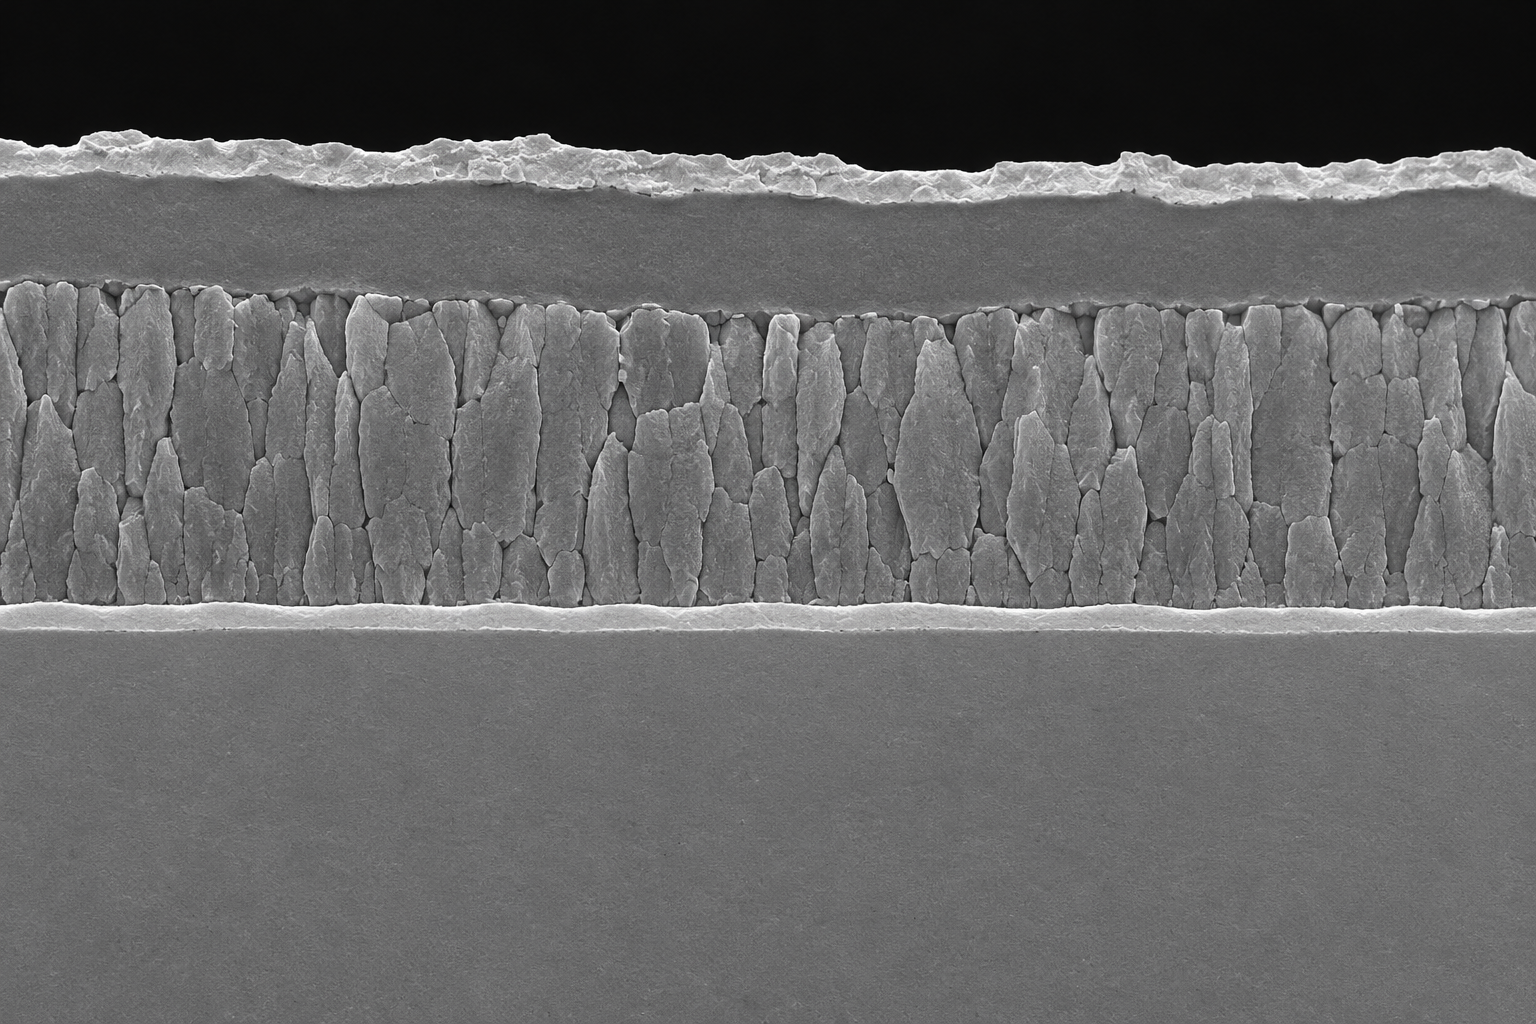
\includegraphics[width=0.78\linewidth]{figures/ch09/ch09-04-sem-like-illustration-base.png}};
\begin{scope}[x={(img.south east)},y={(img.north west)}]
  \node[anchor=south west,fill=white,fill opacity=0.90,text opacity=1,text=black,font=\sffamily\footnotesize,inner sep=2.5pt] at (0.02,0.03) {模型生成示意，非显微图像};
\end{scope}
\end{tikzpicture}
\caption{截面形貌的模型生成示意（面板 b）。本图由图像生成模型绘制，不是显微图像，没有物理比例尺，仅用于示意层序与版式。真实论文中此面板必须是同批器件的实际 SEM 图像，并保留原图与处理记录（见第 8 章）。}\label{fig:ch09-04}
\end{figure}

\subsection*{第四步：初次拼合（v1）的十个问题与修改单}

图~\ref{fig:ch09-06} 复现了“各面板分别做好后直接拖进同一画布”的初稿（v1），红底编号 1–10 标出了画面上的十处具体问题：

\begin{figure}[htbp]\centering
\begin{tikzpicture}
\definecolor{ChNineBad}{HTML}{C0392B}
\node[anchor=south west,inner sep=0] (img) at (0,0) {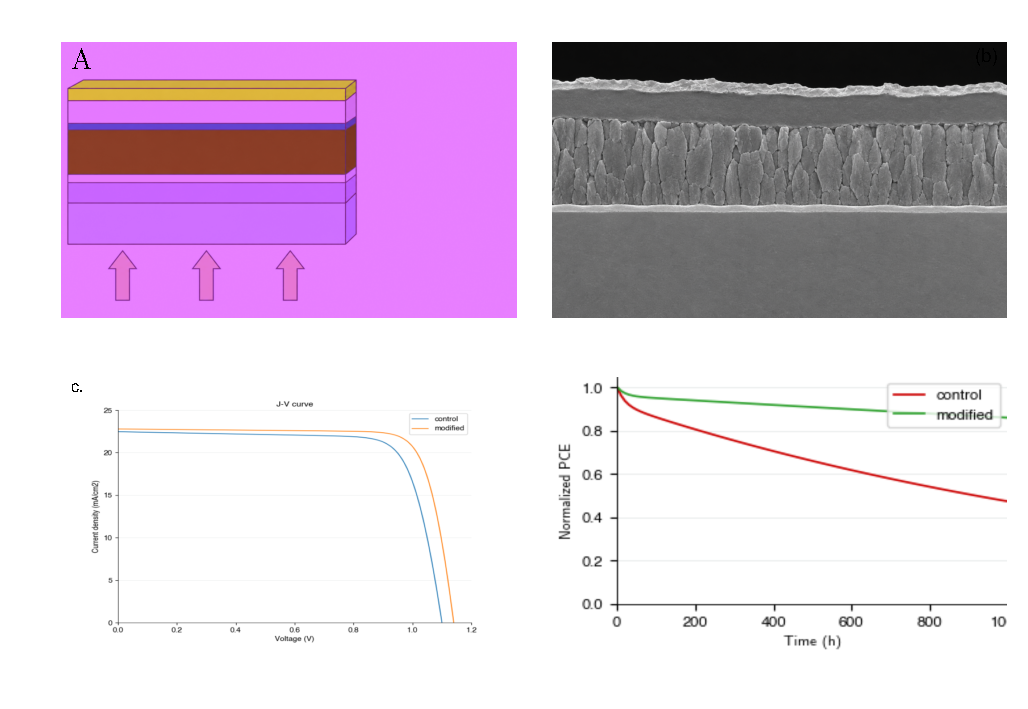
\includegraphics[width=\linewidth]{figures/ch09/ch09-06-assembly-v1-zh.pdf}};
\begin{scope}[x={(img.south east)},y={(img.north west)}]
  \tikzset{
    badnum/.style={draw=white,line width=0.7pt,fill=ChNineBad,text=white,circle,font=\sffamily\bfseries\scriptsize,inner sep=1pt,minimum size=4.0mm},
    badtxt/.style={fill=white,fill opacity=0.88,text opacity=1,text=ChNineBad!90!black,font=\sffamily\scriptsize\bfseries,inner sep=1.2pt,rounded corners=1pt}
  }
  \node[badnum] (b1) at (0.03,0.95) {1};
  \node[badtxt,anchor=west] at (b1.east) {面板字母混用};
  \node[badnum] (b2) at (0.62,0.30) {2};
  \node[badtxt,anchor=west] at (b2.east) {字号不一};
  \node[badnum] (b3) at (0.20,0.70) {3};
  \node[badtxt,anchor=west] at (b3.east) {颜色语义不一致};
  \node[badnum] (b4) at (0.85,0.20) {4};
  \node[badtxt,anchor=east] at (b4.west) {灰度不可分};
  \node[badnum] (b5) at (0.75,0.40) {5};
  \node[badtxt,anchor=west] at (b5.east) {图例压线};
  \node[badnum] (b6) at (0.50,0.08) {6};
  \node[badtxt,anchor=west] at (b6.east) {轴框未对齐};
  \node[badnum] (b7) at (0.75,0.75) {7};
  \node[badtxt,anchor=west] at (b7.east) {b 被拉伸};
  \node[badnum] (b8) at (0.50,0.52) {8};
  \node[badtxt,anchor=west] at (b8.east) {间距不一};
  \node[badnum] (b9) at (0.92,0.92) {9};
  \node[badtxt,anchor=east] at (b9.west) {缺少模拟/模型生成标注};
  \node[badnum] (b10) at (0.30,0.45) {10};
  \node[badtxt,anchor=west] at (b10.east) {面板标题重复图注};
\end{scope}
\end{tikzpicture}
\caption{初次拼合（v1，刻意复现的反例）。编号 1–10 为正文讨论的问题。b 为模型生成示意，非显微图像；c、d 为模拟数据——本版缺少这些面板内标注，正是问题 9。}\label{fig:ch09-06}
\end{figure}

\begin{enumerate}
\item \textbf{面板字母混用且漏标（1）：}a 处为 $14\ \text{pt}$ 衬线大写“A”，b 处为右上角深黑背景中几乎不可见的 $9\ \text{pt}$“(b)”，c 处为“c.”，d 漏标字母。
\item \textbf{字号相差近一倍（2）：}c 按 $8 \times 6\ \text{in}$ 默认尺寸出图后缩入格子，刻度仅约 $4.5\ \text{pt}$；d 按 $84 \times 56\ \text{mm}$、$8\ \text{pt}$ 出图，且右端刻度“1000”被画布边裁成“10”。
\item \textbf{颜色语义不一致（3）：}a 因色相偏移使钝化层变深紫、白底染紫红；c 用默认蓝/橙；d 用红/绿，同一组在三处颜色完全不同。
\item \textbf{灰度不可分（4）：}c、d 两组均为实线，且 d 的红/绿撞色对色觉异常读者不友好。
\item \textbf{图例框压线（5）：}c、d 带边框图例，其中 d 的图例框直接压在绿色改性曲线上。
\item \textbf{坐标轴框未对齐（6）：}c 与 d 的坐标轴左缘错位约 $1.4\ \text{mm}$，底边错位约 $3.2\ \text{mm}$。
\item \textbf{图像被拉伸（7）：}b 以 \texttt{aspect='auto'} 拉伸到与 a 同高，晶粒形貌纵向失真。
\item \textbf{面板间距不一（8）：}网格留白不均，缺少“组间大于组内”的分组层次。
\item \textbf{缺少面板内声明与参考线（9）：}无“模拟数据”“模型生成示意”“不按比例”标注，a 无层名，d 缺 $0.8$ 参考线。
\item \textbf{面板标题重复图注且单位不规范（10）：}c、d 顶部带“J-V curve”“Stability test”标题，c 纵轴单位写成 \texttt{mA/cm2}。
\end{enumerate}

针对这十个问题，逐条开具修改单：

\begin{Prompt}
修改单
1. 面板字母统一为粗体小写 a–d，10 pt，位于各面板左上角外侧，同一基线（画布顶留 5 mm）。
2. c、d 按最终尺寸在 174 × 116 mm 画布上直接重绘，所有文字 8 pt，拼合缩放系数为 1.0。
3. 颜色语义统一：对照 #6E6E6E 虚线，改性 #1B7F86 实线；a 恢复白底原图，钝化层标签用 #1B7F86。
4. 去掉图例框，在曲线内侧空白带直接标注“对照”“改性”（字号 8 pt，颜色同曲线）。
5. 固定四面板左右缘：左列 a、c 为 x = 13–82 mm，右列 b、d 为 x = 101–170 mm；
   c、d 轴框底边均为 y = 11 mm、高 46 mm；末位刻度“1.2”与“1000”右对齐内收。
6. a、b 按原始宽高比置入（宽 69 mm，高 43.2 mm 与 46.0 mm），顶边齐平，不拉伸。
7. 列间距统一 6 mm（另留 13 mm 纵轴走廊）；上下排之间留 8 mm 行距。
8. c、d 右上角加“模拟数据”；b 左下角加“模型生成示意，非显微图像”；
   a 加层名与右下角“不按比例”；d 加 0.8 点线参考线并标“80%”与“T80 约 210 h”。
9. 删除面板内标题；单位统一为 V、mA cm^-2、h。
10. 导出矢量 PDF（pdf.fonttype 42）与 300 dpi PNG；记录每个面板的尺寸与缩放系数。
\end{Prompt}

\subsection*{第五步：修订终稿（v2）与 SciDraw AI 组图工具复现}

按修改单生成的修订版（v2）见图~\ref{fig:ch09-07}。若使用 \scidraw{} 组图工具（\sdtool{multi-panel-figure-maker}）排版同一张图，操作与核对要点如下：

\begin{figure}[htbp]\centering
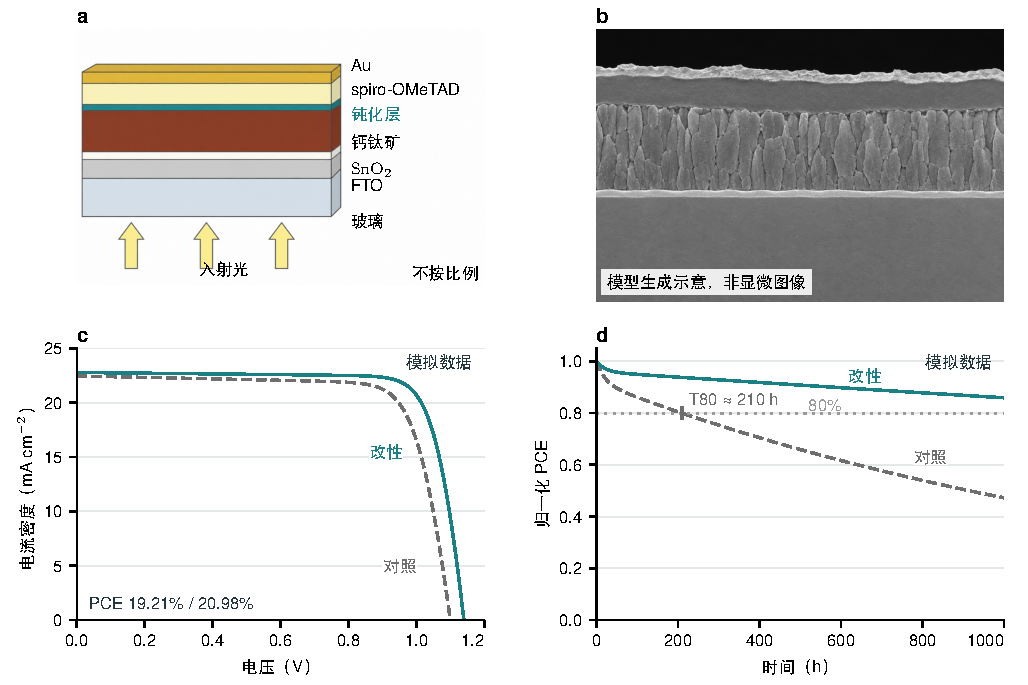
\includegraphics[width=\linewidth]{figures/ch09/ch09-07-assembly-final-zh.pdf}
\caption{修订后的组图（v2）。\textbf{图 2 | 界面钝化对钙钛矿太阳能电池初始性能与运行稳定性的影响（模拟教学数据）。} \textbf{a}，改性器件结构示意（玻璃/FTO/$\text{SnO}_2$/钙钛矿/钝化层/spiro-OMeTAD/Au，光从玻璃侧入射）；对照器件无钝化层；各层厚度不按比例。\textbf{b}，截面形貌示意，由图像生成模型绘制，\textbf{非显微图像}，仅示意层序。\textbf{c}，对照（灰色虚线）与改性（青色实线）器件的 $J\text{--}V$ 曲线，按单二极管模型模拟（AM1.5G，$100\ \text{mW cm}^{-2}$，单一扫描方向，未模拟迟滞）；对照 PCE 19.21\%，改性 20.98\%。\textbf{d}，归一化 PCE 随时间的变化（模拟条件：连续 1 个太阳光照、最大功率点跟踪、氮气、约 $25\ ^\circ\text{C}$）；点线为初始值的 80\%，对照 $T_{80}$ 约 $210\ \text{h}$，改性在 $1000\ \text{h}$ 内未降至 80\%。c、d 每组为一条模拟曲线，不代表器件间分布，未做统计检验。模拟参数与脚本见本书仓库。}\label{fig:ch09-07}
\end{figure}

\begin{enumerate}
\item \textbf{文件交接与期刊预设：}工具间不自动传图，需先将已叠好标签的 \textbf{a}、\textbf{b} PNG 和按终尺寸导出的 \textbf{c}、\textbf{d} PNG 上传至 \texttt{/multi-panel-\allowbreak figure-\allowbreak maker}（当前文档保存在浏览器本地存储中）。选择 Springer 或 Cell 的双栏 $174\ \text{mm}$ 预设与 $2 \times 2$ 网格，开启自动编号。注意编号样式跟随期刊预设（Springer 预设为小写 \textbf{a}，Cell 预设为大写 \textbf{A}），投稿前须对照作者指南核实。
\item \textbf{导出格式与能力边界：}导出包含 TIFF、PNG、PDF、PPTX 与处理记录的 ZIP 包。PPTX 中面板位图与编号文字可分别编辑，但面板内部文字不可编辑；组图工具不提供 AI 自动规划布局、修改面板内文字或将位图转为可编辑矢量，这些必须在生成单面板时解决。
\item \textbf{读处理记录核算实际字号与有效分辨率：}处理记录给出各面板在图中的毫米尺寸和缩放系数。若面板 \textbf{c} 原图按 $84\ \text{mm}$ 宽、$8\ \text{pt}$ 出图，但在组图中被放成 $80\ \text{mm}$ 宽（缩放系数 $80/84 \approx 0.952$），实际字号 $= 8 \times 80 / 84 \approx 7.6\ \text{pt}$，就低于 $8\ \text{pt}$ 要求；正确做法是回到脚本按格子实际尺寸重出，而不是在组图工具里放大。位图有效分辨率按“源像素宽 $\div$ 印刷英寸宽”计算：在图~\ref{fig:ch09-07} 中，面板 \textbf{a}（$1586\ \text{px}$）与面板 \textbf{b}（$1536\ \text{px}$）在 $69.0\ \text{mm}$（$2.717\ \text{in}$）宽下的有效分辨率分别为 $1586 / 2.717 \approx 584\ \text{ppi}$ 与 $1536 / 2.717 \approx 565\ \text{ppi}$，均远高于 $300\ \text{ppi}$ 的常规要求。
\end{enumerate}

\section{图注：AI 起草，作者补全}

一段完整的组图图注包含五个构件：总标题句、逐面板说明（含视觉编码定义）、关键实验或模拟条件、样本量与统计方法、数据性质与来源声明。

把终稿 PNG 上传至 \scidraw{} 图注辅助工具（\sdtool{figure-legend}）并选择输出语言后，工具只看图片像素，输出一段 40–120 词的描述性图注草稿。例如预期草稿形态通常为：“钙钛矿太阳能电池的器件结构、截面形貌与光伏性能。(a) 器件层状结构示意。(b) 器件截面图像。(c) 对照与改性器件的 J–V 曲线。(d) 归一化 PCE 随时间的变化。”

按设计原则，\sdtool{figure-legend} 绝不编造画面中看不到的样本量、$p$ 值、统计检验、处理条件或化学分子式。作者拿到草稿后，必须把“看图可见的”与“必须知道的”分开核对（图~\ref{fig:ch09-08}）：

\begin{figure}[htbp]\centering
\resizebox{\linewidth}{!}{% FIG ch09-08 legend drafting (Chinese)
\begin{tikzpicture}[
  x=1mm, y=1mm,
  font=\sffamily\scriptsize,
  text=BookInk,
  col/.style={draw=BookInk!45, line width=0.4pt, rounded corners=1pt, inner sep=2mm, align=justify, text width=78mm},
  hi/.style={fill=BookPale, draw=BookTeal, line width=0.8pt, rounded corners=1pt, inner sep=1.5mm},
  tag/.style={font=\tiny\bfseries, text=BookTeal, anchor=east},
]
  \node[font=\small\bfseries, anchor=west] at (0, 118) {图注起草对照};
  \node[col, anchor=north west] (draft) at (0, 112) {
    \textbf{/figure-legend 草稿（实测原文）}\par\vspace{1mm}
    \fbox{\parbox[t]{72mm}{\centering 待实测，见 \texttt{provenance/ch09/figure-legend-draft-zh.txt}}}
  };
  \node[col, anchor=north west] (final) at (88, 112) {
    \textbf{作者补全版（节选）}\par\vspace{1mm}
    \tikz{\node[hi, text width=72mm, anchor=west] (t1) at (0,0) {
      \textbf{图 2 |} 界面钝化对钙钛矿太阳能电池初始性能与运行稳定性的影响（\textbf{模拟教学数据}）。
    }; \node[tag] at (-1,0) {【数据性质】};}\par
    \tikz{\node[hi, text width=72mm, anchor=west] (t2) at (0,0) {
      \textbf{b}，截面形貌示意，由图像生成模型绘制，\textbf{非显微图像}……
    }; \node[tag] at (-1,0) {【定义】};}\par
    \tikz{\node[hi, text width=72mm, anchor=west] at (0,0) {
      c、d 每组为一条模拟曲线，未做统计检验；脚本见 \texttt{sim\_perovskite.py}。
    }; \node[tag] at (-1,0) {【来源】};}
  };
  \node[anchor=west, text=BookInk!70] at (0, 4) {
    删改示例：\sout{截面图像} $\rightarrow$ 模型生成示意，非显微图像
  };
\end{tikzpicture}
}
\caption{图注由 AI 起草、作者补全。左：\sdtool{figure-legend} 根据图像生成的草稿框；右：作者补全版，高亮部分是图像中看不到、必须由作者提供的信息。}\label{fig:ch09-08}
\end{figure}

\begin{itemize}
\item \textbf{删改视觉误判：}草稿可能把面板 \textbf{b} 写成“截面图像/SEM 图像”，必须改为“截面形貌示意，由图像生成模型绘制，非显微图像，仅示意层序”。
\item \textbf{补齐五类背景信息：}(1) \textbf{【数据性质】}模拟教学数据、各层厚度不按比例、非显微图像；(2) \textbf{【器件与条件】}七层结构与光入射方向、单二极管模型（AM1.5G，$100\ \text{mW cm}^{-2}$，单一扫描方向，未模拟迟滞——真实钙钛矿电池存在反常迟滞，须按 Snaith 等 2014 报告扫描方向与速率）、连续 1 个太阳光照、最大功率点跟踪、氮气、约 $25\ ^\circ\text{C}$（若标注 ISOS-L-1 等标准代号，须对照 Khenkin 等 2020 核实全部测试条件）；(3) \textbf{【样本与统计】}对照 PCE $19.21\%$、改性 $20.98\%$，声明每组一条模拟曲线、不代表器件间分布、未做统计检验；(4) \textbf{【定义】}点线为初始值的 80\%，对照 $T_{80}$ 约 $210\ \text{h}$，改性在 $1000\ \text{h}$ 内未降至 80\%；(5) \textbf{【来源】}模拟参数与脚本位置（完整终稿图注见图~\ref{fig:ch09-07}）。
\end{itemize}

在真实实验论文中，作者可按如下填空模板补齐样本量与统计信息（\texttt{【】}内由作者据实验记录填入）：

\begin{BookNote}
\textbf{真实论文版图注模板：} \textbf{c}，……代表性器件的 $J\text{--}V$ 曲线（反向扫描，【扫描速率】$\text{mV s}^{-1}$，【有效面积】$\text{cm}^2$，掩膜【有/无】）；插表为 $n =$【器件数】个器件、来自【批次数】个独立批次的光伏参数（均值 $\pm$ 标准差）。\textbf{d}，……$n =$【器件数】个未封装器件，【气氛】，【温度】$^\circ\text{C}$，阴影为【标准差/标准误/范围】；$T_{80}$ 定义为【首次降至初始值 80\% 的时间/拟合值】。统计检验：【检验方法】，【$P$ 值】。
\end{BookNote}

交付前，结合 \sdtool{figure-checker} 与脚本断言完成八项终审核验（表~\ref{tab:ch09-verify}）。

\begin{table}[htbp]\centering\footnotesize
\setlength{\tabcolsep}{3pt}
\renewcommand{\arraystretch}{1.15}
\caption{本章案例终稿（图~\ref{fig:ch09-07}）的八项交付前核验。}\label{tab:ch09-verify}
\begin{tabularx}{\linewidth}{@{}>{\raggedright\arraybackslash}p{26mm}YY@{}}
\toprule
\textbf{核验项} & \textbf{检查方法} & \textbf{终稿实测结果} \\
\midrule
数值一致性 & 脚本断言比对数据表与图面、图注数字 & PCE $19.21\%$/$20.98\%$、$T_{80}=210\ \text{h}$/$>1000\ \text{h}$ 完全一致 \\
100\% 缩放字号 & 在 $174\ \text{mm}$ 宽下查 PDF 字体属性或量大写字母高（$8\ \text{pt} \approx 2.0\ \text{mm}$） & 面板字母 $10\ \text{pt}$ 粗体，其余文字均 $8\ \text{pt}$，无越界裁切 \\
坐标轴框对齐 & 检验四框毫米坐标（\texttt{ax.get\_position()} 断言） & a/c 对齐 $13\text{--}82\ \text{mm}$，b/d 对齐 $101\text{--}170\ \text{mm}$，c/d 底边均 $11\ \text{mm}$ \\
图像宽高比 & 对比置入框与原图宽高比 & a（$69.0 \times 43.2\ \text{mm}$）、b（$69.0 \times 46.0\ \text{mm}$）误差 $< 0.1\%$ \\
灰度与色觉 & 灰度转换及 Machado（2009）色觉模拟 / \sdtool{figure-checker} & 灰虚线、青实线与浅灰点线在灰度与色觉模拟下均可区分 \\
面板内声明 & 目视检查四面板内部声明文字 & “不按比例”“模型生成示意，非显微图像”“模拟数据”均清晰可见 \\
缩放系数与 ppi & 查处理记录缩放系数，算源像素 $\div$ 印刷英寸宽 & c、d 缩放系数 $1.0$；a 约 $584\ \text{ppi}$、b 约 $565\ \text{ppi}$ \\
图注可溯源 & 逐项核对图注数字与说明出处 & 全部来自数据文件与脚本设定，无图中不可见且无依据的内容 \\
\bottomrule
\end{tabularx}
\end{table}

\section{AI 在这一步能做什么与不能做什么}

组图与图注各环节中 AI、确定性工具与作者的职责边界汇总于表~\ref{tab:ch09-01}。

\begin{table}[htbp]\centering\footnotesize
\setlength{\tabcolsep}{3pt}
\renewcommand{\arraystretch}{1.15}
\caption{AI 在组图环节能做、不能做与作者要核对的内容。}\label{tab:ch09-01}
\begin{tabularx}{\linewidth}{@{}>{\raggedright\arraybackslash}p{18mm}YYY@{}}
\toprule
\textbf{环节} & \textbf{AI 能做} & \textbf{AI 不能做} & \textbf{作者要核对} \\
\midrule
面板分工 & 根据任务书列出面板分工与顺序候选；指出与主问题无关的面板 & 判断证据是否足以支持结论；决定哪些数据可以不放 & 每个面板回答的子问题；被移出的面板去向（补充材料） \\
网格规划 & 按期刊宽度换算格子尺寸；写 \texttt{gridspec} / 固定轴框的脚本 & 理解面板内容的科学重要性来分配面积（当前组图工具不做 AI 布局规划） & 最终尺寸、宽高比不变、分组留白 \\
示意面板 & 生成无字底图（结构、层序、示意形貌） & 保证层序、比例与真实器件一致；生成可作证据的形貌图 & 层数与顺序；颜色语义；“示意/模型生成”标注 \\
数据面板 & 按规范写绘图脚本；统一 \texttt{rcParams} & 选择或修改数据；补出没有的误差带 & 数值来自数据文件；字号在最终尺寸下达标；灰度可分 \\
排版与导出 & \scidraw{} 组图工具：网格、跨行列、自动编号、期刊尺寸预设、处理记录、TIFF/PNG/PDF/PPTX & 修改面板内部文字；统一已经栅格化的面板字体；把位图变成可编辑矢量 & 处理记录中的缩放系数与有效分辨率；编号样式符合期刊 \\
图注 & \sdtool{figure-legend} 起草看图可见的描述 & 写样本量、批次、测试条件、统计方法、数据性质（工具按设计不编造） & 补全 $n$、条件、统计、定义、来源；删去误判（如把示意写成 SEM） \\
技术检查 & \sdtool{figure-checker} 检查格式、分辨率、灰度与色觉风险 & 审核科学结论或统计选择 & 检查报告之外的科学核验 \\
\bottomrule
\end{tabularx}
\end{table}

\section{本章检查清单}

\begin{itemize}
\item 写下了组图的主问题，每个面板都有明确的子问题或证据角色；无关面板已移出。
\item 画布按目标期刊最终宽度（本例 $174\ \text{mm}$）设定，高度在限制内。
\item 数据面板按最终格子尺寸出图，拼合时缩放系数为 $1.0$（或已据此换算实际字号）。
\item 全图一种字体；最小字号满足期刊要求；面板字母样式、大小、位置统一。
\item 同组数据面板的坐标轴框对齐；面板间距一致，组间留白大于组内。
\item 同一组别在所有面板中颜色相同；颜色之外还有线型或标注区分；灰度与色觉模拟通过。
\item 图像面板保持原宽高比，没有拉伸。
\item 模拟数据、模型生成图样、不按比例等声明写在\textbf{面板内}，也写在图注中。
\item 图注包含：标题句、逐面板说明、样本量与重复、测试条件、统计方法与误差含义、定义（如 $T_{80}$）、数据与代码来源。
\item 处理记录、脚本、原始数据与组图导出文件一并保存；从数据脚本到组图工具的文件交接有记录。
\end{itemize}

\section{练习}

\begin{enumerate}
\item \textbf{面板分工（纸笔）。} 取你最近的一张论文组图，写出它的主问题和每个面板的子问题；找出一个不直接回答主问题的面板，说明它应该留下、合并还是移到补充材料。
\item \textbf{最终尺寸检查（脚本）。} 用本章配套的数据面板绘图脚本把面板 \textbf{c} 分别按 $\text{figsize}=(8,6)\ \text{in}$ 和 $84 \times 56\ \text{mm}$ 出图，都放进 $84\ \text{mm}$ 宽的格子里，计算两种情况下刻度文字的实际字号；再把对照曲线改为与改性同为实线，转灰度，记录能否区分。
\item \textbf{\scidraw{} 实操。} 把本章提供的四个面板 PNG 导入 \texttt{/multi-panel-\allowbreak figure-\allowbreak maker}，分别选 Springer 与 Cell 的 $174\ \text{mm}$ 预设，比较编号样式的差别；导出 ZIP，从处理记录中读出 \textbf{c} 的缩放系数并换算实际字号。然后把导出的 PNG 上传 \sdtool{figure-legend}，保存草稿原文，按第 9.6 节的类别逐项补全图注。附加：阅读 Burkitt 等（2018）图 6（CC BY 4.0，真实 SEM 图），列出一张真实 SEM 面板在图中和图注里分别需要提供的信息（仪器、视角、比例尺、样品与工艺），并说明为什么不能把它放进本章的 Figure 2。
\end{enumerate}

\section*{参考文献}

\begin{itemize}
\item Burkitt D, Searle J, Watson T. Perovskite solar cells in N-I-P structure with four slot-die-coated layers. \textit{Royal Society Open Science}. 2018;5(5):172158. doi:10.1098/rsos.172158
\item Crameri F, Shephard GE, Heron PJ. The misuse of colour in science communication. \textit{Nature Communications}. 2020;11:5444. doi:10.1038/s41467-020-19160-7
\item Jambor H, Antonietti A, Alicea B, et al. Creating clear and informative image-based figures for scientific publications. \textit{PLOS Biology}. 2021;19(3):e3001161. doi:10.1371/journal.pbio.3001161
\item Khenkin MV, Katz EA, Abate A, et al. Consensus statement for stability assessment and reporting for perovskite photovoltaics based on ISOS procedures. \textit{Nature Energy}. 2020;5(1):35--49. doi:10.1038/s41560-019-0529-5
\item Kojima A, Teshima K, Shirai Y, Miyasaka T. Organometal halide perovskites as visible-light sensitizers for photovoltaic cells. \textit{Journal of the American Chemical Society}. 2009;131(17):6050--6051. doi:10.1021/ja809598r
\item Machado GM, Oliveira MM, Fernandes LAF. A physiologically-based model for simulation of color vision deficiency. \textit{IEEE Transactions on Visualization and Computer Graphics}. 2009;15(6):1291--1298. doi:10.1109/TVCG.2009.113
\item Nature Portfolio. Preparing figures -- our specifications. \url{https://research-figure-guide.nature.com/figures/preparing-figures-our-specifications/} (accessed 2026-10-29).
\item Rougier NP, Droettboom M, Bourne PE. Ten simple rules for better figures. \textit{PLoS Computational Biology}. 2014;10(9):e1003833. doi:10.1371/journal.pcbi.1003833
\item Snaith HJ, Abate A, Ball JM, et al. Anomalous hysteresis in perovskite solar cells. \textit{The Journal of Physical Chemistry Letters}. 2014;5(9):1511--1515. doi:10.1021/jz500113x
\item Wong B. Points of view: Color blindness. \textit{Nature Methods}. 2011;8(6):441. doi:10.1038/nmeth.1618
\end{itemize}

% TODO: provenance/ch09/figure-legend-draft-zh.txt 尚未生成（figures/ch09/ch09-08-legend-drafting-zh.tex 左栏当前为“待实测”占位框）。
% TODO: figures/ch09/ch09-03-device-structure-zh.png 与 figures/ch09/ch09-04-sem-like-illustration-zh.png 独立预叠加位图未单独生成（本章已按规范使用底图 + TikZ 叠加展示，合成图 ch09-07 已直接内置叠加）。
% TODO: figures/ch09/ch09-05-data-panels-zh.pdf 为 ch09_plot_utils.py 调整标注坐标前导出的版本（右下角“对照”“改性”标签仍在曲线末点重叠），重跑 scripts/ch09_panels.py 后可与 ch09-07 同步。
